\documentclass[11pt,a4paper]{article}

\usepackage[margin=1in]{geometry}
\usepackage{amsmath,amssymb}
\usepackage{booktabs}
\usepackage{graphicx}
\usepackage{hyperref}
\usepackage{microtype}
\usepackage{enumitem}
\usepackage{listings}
\usepackage{xcolor}
\usepackage{caption}
\usepackage{subcaption}
\usepackage[numbers,sort&compress]{natbib}

\hypersetup{
  colorlinks=true,
  linkcolor=blue,
  citecolor=blue,
  urlcolor=blue
}

\lstdefinestyle{cli}{
  basicstyle=\ttfamily\small,
  breaklines=true,
  frame=single,
  backgroundcolor=\color{gray!8},
  showstringspaces=false
}

\lstdefinestyle{pipeline}{
  basicstyle=\ttfamily\small,
  breaklines=false,
  frame=single,
  backgroundcolor=\color{gray!8}
}

\title{%
  Phase-Aware IQ Autoencoding for ADS-B Mode S:\\
  Synthetic Blind Source Separation, Real-World Constraints,\\
  and Conservative Deployment via Model--Raw Blending
}

\author{%
  {\large Anuvind Saj}\\[0.75em]
  \textit{Technical Report --- July 2026}
}

\date{}

\begin{document}
\maketitle

\begin{center}
  \small\itshape
  Experimental phase closed --- July 2026.\\[0.25em]
  Code-verified results from the \texttt{adsb\_autoencoder} project.
\end{center}
\vspace{1em}

\begin{abstract}
Automatic Dependent Surveillance--Broadcast (ADS-B) Mode~S receivers typically
decode pulse-position-modulated messages from a magnitude-only envelope,
discarding phase information that could resolve co-channel collisions. I
present a phase-aware 1D U-Net autoencoder operating directly on complex
baseband IQ samples at 2~MSPS, trained for denoising and blind source
separation (BSS) of overlapping aircraft transmissions. Synthetic pre-training
demonstrates rapid convergence and visually convincing collision separation in
simulation. Supervised fine-tuning on 152{,}343 pairs extracted from 406~GB of
RTL-SDR captures yields partial success: the v1 checkpoint recovers 116
CRC-valid frames (7.3\%) from a held-out in-distribution capture versus zero
from synthetic-only weights, while suppressing the estimated noise floor below
raw hardware levels. Subsequent training iterations (v2--v4) achieve lower
validation loss but regress on the downstream metric that matters---CRC-valid
frame count---due to objective mismatch, collision-augmentation
over-suppression, and out-of-distribution capture statistics. Pipeline
validation (\texttt{--identity} mode) preserves 314/314 decodable frames on an
out-of-distribution test capture, isolating failures to learned weights rather
than streaming infrastructure. A conservative deployment strategy mixing 5\%
model output with 95\% raw signal preserves 89--100\% of raw decodability
across three independent real captures. I conclude that IQ autoencoding for
ADS-B is feasible in simulation but requires decoder-aligned training
objectives, real collision ground truth, and domain coverage before
standalone full-strength deployment is viable.

\medskip
\noindent\textbf{Keywords:} ADS-B, Mode~S, software-defined radio, blind source
separation, U-Net, IQ processing, RTL-SDR
\end{abstract}

%=============================================================================
\section{Introduction}
%=============================================================================

ADS-B Mode~S transponders broadcast aircraft identity, position, and velocity
on 1090~MHz using on-off keying with pulse-position modulation (PPM). Ground
receivers such as \texttt{dump1090}~\cite{dump1090fa} demodulate these messages by thresholding a
magnitude envelope derived from IQ samples. For isolated transmissions this
approach is adequate. In congested airspace, however, multiple aircraft may
transmit on the same frequency within the same 120~\textmu s frame
window---a \emph{co-channel collision}. Because the magnitude of a sum of
phasors is not the sum of magnitudes, constructive and destructive phase
interference corrupts PPM bit positions and causes CRC failures. Reported
collision rates range from 5--15\% in general traffic and can exceed 30\% near
major airports.

Retaining both in-phase ($I$) and quadrature ($Q$) channels through processing
preserves geometric structure invisible to magnitude-only decoders: each
aircraft's phasor traces a spiral on the complex plane at an angular velocity
determined by its unique oscillator offset relative to the receiver's local
oscillator. When two signals superimpose, their distinct rotation rates produce
a \emph{beating envelope}---a Lissajous trajectory that encodes the presence of
two sources and provides a discriminant for blind source separation.

This work investigates whether a deep neural network can exploit that phase
geometry to (1)~denoise RTL-SDR captures while preserving sub-microsecond pulse
timing, and (2)~reconstruct a primary aircraft's transmission from a two-source
collision---all without modifying legacy decoders. Processed IQ is written back
to standard RTL-SDR \texttt{uint8} interleaved format and fed to unmodified
\texttt{dump1090}, making downstream decode success the primary evaluation
metric.

\subsection{Contributions}

\begin{enumerate}[leftmargin=*]
  \item A \textbf{physics-aligned data generator} (\texttt{generator.py})
        synthesising 240-sample Mode~S frames at 2.0~MSPS with exact PPM grid
        alignment, hardware impairments, and collision superposition.
  \item A \textbf{phase-aware 1D U-Net} (\texttt{IQAutoencoder}, 4.19M
        parameters) with a composite IQ/magnitude/circular-phase loss designed
        for OOK carrier structure.
  \item A \textbf{supervised labelling pipeline} (\texttt{extract\_labels.py})
        extracting 152{,}343 training pairs from real RTL-SDR bursts by
        CRC-gated re-synthesis.
  \item \textbf{Hybrid collision augmentation} (\texttt{supervised\_dataset.py})
        superimposing synthetic interferers onto real captures, with documented
        failure modes when misconfigured.
  \item A \textbf{streaming inference bridge} (\texttt{live\_bridge.py}) with
        overlap-add synthesis, global DC warmup, and validated
        \texttt{--identity} / \texttt{--blend} modes.
  \item An \textbf{honest negative-result analysis} documenting
        validation-loss versus decode-metric divergence, domain shift, and the
        partial deployability of a 5\% model blend.
\end{enumerate}

\subsection{What This Paper Does Not Claim}

This work does \textbf{not} claim that full-strength model inference improves ADS-B
frame recovery over raw reception on real captures. It does \textbf{not}
demonstrate live collision resolution on field data. It does \textbf{not} present a
production-ready standalone denoiser. Success is defined as preserving
decodability under conservative blending while documenting why full-strength
deployment fails.

%=============================================================================
\section{Background}
%=============================================================================

\subsection{Mode S PPM and Decoder Failure at Collisions}

A Mode~S long squitter occupies 120~\textmu s: an 8~\textmu s preamble (four
0.5~\textmu s pulses) followed by 112 data bits, each encoded as a pulse in the
first or second half of a 1~\textmu s bit cell~\cite{rtca_do260b}. Decoders locate preambles, slice
bit windows, and validate a 24-bit CRC.

When two signals $s_A(t)$ and $s_B(t)$ overlap, the received sample is their
complex sum $r(t) = s_A(t) + s_B(t)$. The magnitude envelope $|r(t)|$ depends
on the instantaneous phase difference $\Delta\phi(t)$:
\begin{itemize}[leftmargin=*]
  \item \textbf{Constructive} ($\Delta\phi \approx 0$): pulses appear amplified.
  \item \textbf{Destructive} ($\Delta\phi \approx \pi$): pulses may vanish entirely.
\end{itemize}
Standard threshold detectors see garbled pulse positions; CRC checks fail. This
is an information-theoretic limitation of magnitude-only processing, not
merely a threshold tuning problem.

\subsection{Beating as a BSS Discriminant}

After downconversion, each aircraft appears at a unique frequency offset $f_a,
f_b$ relative to the receiver IF. Their phasors rotate at different rates;
during overlapping pulse windows the combined trajectory oscillates at the beat
frequency $f_{\mathrm{beat}} = |f_a - f_b|$. In IQ space, collision events
produce characteristic Lissajous figures whose angular-velocity difference is
the primary feature available for source separation---provided phase is
preserved through the processing chain.

\subsection{RTL-SDR Impairments}

RTL2832U dongles use zero-IF architecture, introducing DC offset, thermal AWGN,
phase jitter, and slow frequency drift. Real-world noise additionally includes
1/$f$ flicker, IQ imbalance, intermodulation, and multipath fading---effects
not fully captured by simple AWGN models. Our synthetic generator and labelling
pipeline model DC offset, AWGN, phase jitter, and linear drift; real texture
gaps remain a documented limitation (Section~\ref{sec:discussion}).

\subsection{Sampling Rate: Why 2.0~MHz}

ADS-B PPM uses 0.5~\textmu s bit halves. At \textbf{2.0~MSPS}, each bit half
occupies exactly one sample:

\begin{table}[htbp]
  \centering
  \caption{PPM grid alignment at 2.0~MSPS.}
  \label{tab:ppm-grid}
  \begin{tabular}{@{}lc@{}}
    \toprule
    Quantity & Value \\
    \midrule
    Sample period & 0.5~\textmu s \\
    Preamble samples & 16 \\
    Data bit samples & 2 \\
    Frame length & 240 samples \\
    \bottomrule
  \end{tabular}
\end{table}

At 2.4~MSPS, bit boundaries fall between samples, forcing the network to
learn fractional alignment implicitly. The 2.0~MHz rate makes the PPM grid and
tensor grid \textbf{identical}---a deliberate design constraint, not a
compromise (Figure~\ref{fig:ppm-grid}).

\begin{figure}[htbp]
  \centering
  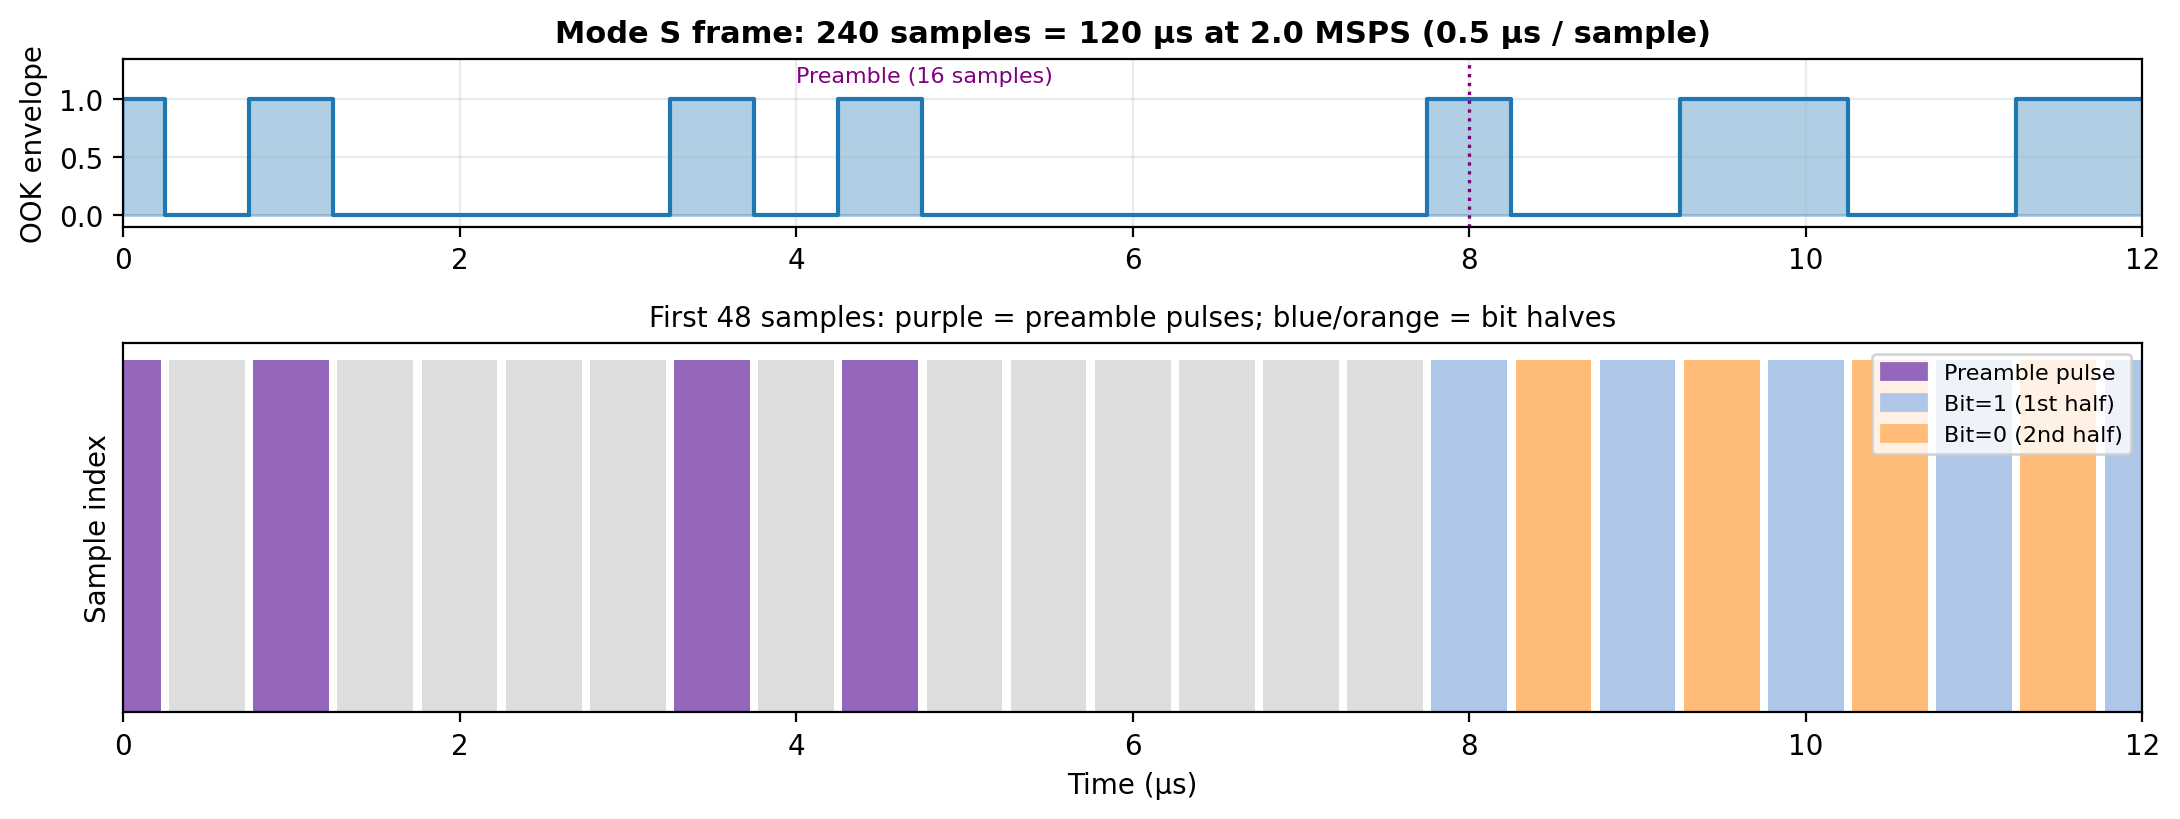
\includegraphics[width=\linewidth]{figures/fig_ppm_grid.png}
  \caption{Mode S OOK envelope and sample-level PPM grid at 2.0~MSPS. Each
  0.5~\textmu s bit half maps to exactly one sample; the preamble occupies 16
  samples.}
  \label{fig:ppm-grid}
\end{figure}

%=============================================================================
\section{System Overview}
%=============================================================================

\subsection{Hardware and Collection}

\begin{table}[htbp]
  \centering
  \caption{Hardware and collection infrastructure.}
  \label{tab:hardware}
  \begin{tabular}{@{}ll@{}}
    \toprule
    Component & Specification \\
    \midrule
    Antenna & Custom 8-segment coaxial collinear (CoCo), 1090~MHz \\
    Receiver & RTL-SDR (RTL2832U) \\
    Edge nodes & Raspberry Pi 3B (collection), Pi 4 (inference target) \\
    Training & Apple Silicon MacBook (MPS acceleration) \\
    Storage & MinIO object store on Pi 4 + 1~TB SSD \\
    Sites & \texttt{rpi\_east}, \texttt{rpi\_west} --- independent orientations \\
    \bottomrule
  \end{tabular}
\end{table}

Captures are recorded at 2~MSPS as interleaved \texttt{uint8} I/Q binaries.
The ML collector (\texttt{ml\_data\_collector.py}) records 30-second bursts with
gain rotation across $\{28, 32, 36, 40, 44\}$~dB, uploading to a dedicated
MinIO bucket. \textbf{406~GB} was collected across June 2026 sessions before an
OOM halt; \textbf{152{,}343} supervised pairs were extracted from 785 label
files covering \textbf{2{,}016} unique ICAO addresses.

\subsection{End-to-End Pipeline}

\begin{lstlisting}[style=pipeline]
RTL-SDR capture (.bin / .npy)
    -> extract_labels.py  ->  supervised pairs (.npz)
    -> train_supervised.py  ->  checkpoint (.pt)
    -> live_bridge.py  ->  processed .bin
    -> compare_decodings.py / dump1090  ->  CRC-valid frame count
\end{lstlisting}

The evaluation metric throughout this report is \textbf{CRC-valid Mode~S frame
count} and \textbf{unique aircraft (ICAO) count}---not training loss, noise
floor estimates, or preamble candidate counts alone
(Figure~\ref{fig:pipeline}).

\begin{figure}[htbp]
  \centering
  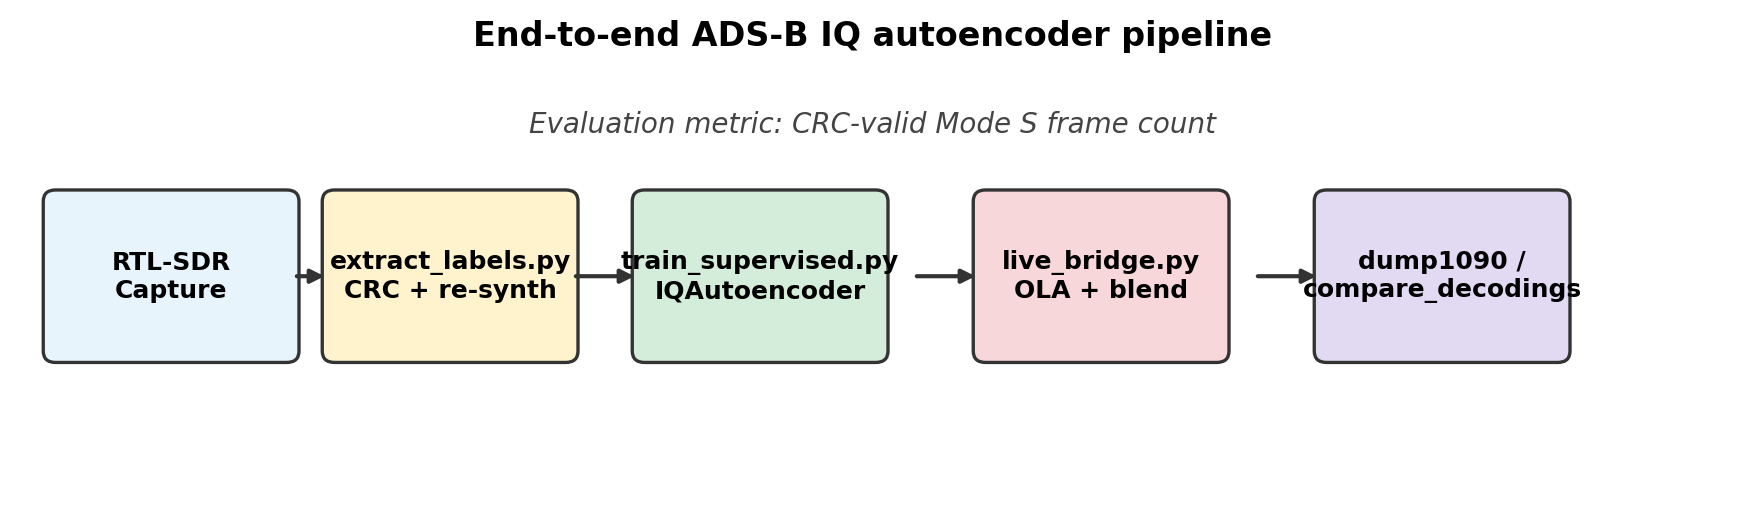
\includegraphics[width=\linewidth]{figures/fig_pipeline.png}
  \caption{End-to-end pipeline from RTL-SDR capture through supervised training
  and streaming inference to CRC-gated evaluation.}
  \label{fig:pipeline}
\end{figure}

%=============================================================================
\section{Method}
%=============================================================================

\subsection{Synthetic Data Generation}

\texttt{ADSBSignalGenerator} constructs frames from first principles:
\begin{enumerate}[leftmargin=*]
  \item \textbf{PPM envelope} --- preamble pulses at sample indices
        $\{0, 2, 7, 9\}$; data bits encoded as pulses in the first or second
        sample of each 2-sample bit cell.
  \item \textbf{Phase accumulator} --- continuous phase
        $\phi(n) = 2\pi f_{\mathrm{offset}} n T_s + \phi_0$ over all 240
        samples, including silence gaps (phase continuity contract).
  \item \textbf{IQ synthesis} ---
        $\mathrm{IQ}(n) = A \cdot e^{j\phi(n)} \cdot \mathrm{envelope}(n)$.
  \item \textbf{Impairments} --- applied in order: frequency drift, phase
        jitter, AWGN, DC offset.
\end{enumerate}

\textbf{Collision synthesis} linearly superimposes two aircraft signals:
\texttt{composite = clean\_a + shifted\_b}. Frequency offsets are drawn from
$\pm 50$~kHz with minimum 8~kHz separation to ensure at least one beat cycle
within 240 samples. Training batches use 25\% collision / 75\% single-aircraft
examples during synthetic pre-training.

\subsection{Supervised Labelling from Real Captures}

\texttt{extract\_labels.py} processes real \texttt{.npy} burst files:
\begin{enumerate}[leftmargin=*]
  \item Remove DC via full-burst mean subtraction.
  \item Detect Mode~S preambles with adaptive thresholding.
  \item Decode bits and validate CRC.
  \item Estimate amplitude, initial phase, and frequency offset from preamble
        pulse phases.
  \item Re-synthesise a clean target frame via \texttt{generator.py}.
\end{enumerate}

Each valid pair consists of a \textbf{real noisy 240-sample window} (input) and
a \textbf{mathematically ideal re-synthesised frame} (target). This is the
project's central training proxy---and its central limitation: the target is
not what the antenna actually received (Section~\ref{sec:constraints}).

\subsection{Hybrid Collision Augmentation}

Because CRC-passing collisions are virtually absent in real data,
\texttt{SupervisedIQDataset} optionally superimposes a synthetic second
aircraft onto real inputs with probability $p$:
\begin{equation}
  x_{\mathrm{aug}}(n) = x_{\mathrm{real},A}(n) + s_{\mathrm{synthetic},B}(n),
  \qquad y = \hat{s}_{\mathrm{clean},A}(n).
  \label{eq:augment}
\end{equation}

Interferer parameters are calibrated relative to signal~A's estimated amplitude,
with frequency offset constrained $\geq 8$~kHz from~A, random initial phase,
random payload, and integer time offset $\in [-24, +24]$ samples covering
partial preamble overlaps.

\textbf{Critical design lesson (v2 regression):} A 30\% augmentation rate with
a \textbf{noise-free} synthetic interferer taught the model to suppress clean
structured patterns---including the primary aircraft after RMS normalisation.
v3 reduced the rate to 10\% and added 20~dB AWGN to the interferer; v4 disabled
augmentation entirely for a denoising-only retrain.

\subsection{Network Architecture}

\textbf{IQAutoencoder} --- U-Net 1D convolutional autoencoder~\cite{ronneberger2015unet}
(\texttt{model.py}):

\begin{table}[htbp]
  \centering
  \caption{IQAutoencoder configuration.}
  \label{tab:architecture}
  \begin{tabular}{@{}ll@{}}
    \toprule
    Parameter & Value \\
    \midrule
    Input shape & $(B, 2, 240)$ --- $I$ and $Q$ channels \\
    Base channels & 64 \\
    Depth & 4 encode/decode stages \\
    Bottleneck & $2\times$ Conv1d at $(B, 512, 15)$ \\
    Parameters & 4{,}186{,}242 \\
    \bottomrule
  \end{tabular}
\end{table}

Skip connections preserve sample-level pulse timing. The encoder downsamples
$240 \to 15$; the decoder upsamples back to 240 with skip fusion. A $1\times 1$
output head produces unbounded IQ values. U-Net was chosen over a plain
autoencoder because PPM decoding requires $\pm 0.5$~\textmu s pulse fidelity
that bottleneck-only decoders blur.

\subsection{Phase-Aware Loss Function}

\begin{equation}
  \mathcal{L}_{\mathrm{total}} =
  w_{iq}\mathcal{L}_{iq} +
  w_{\mathrm{mag}}\mathcal{L}_{\mathrm{mag}} +
  w_{\mathrm{phase}}\mathcal{L}_{\mathrm{phase}}.
  \label{eq:loss}
\end{equation}

\begin{itemize}[leftmargin=*]
  \item $\mathcal{L}_{iq}$ --- channel MSE on raw $I/Q$.
  \item $\mathcal{L}_{\mathrm{mag}}$ --- MSE on magnitude envelopes, enforcing
        on/off pulse structure.
  \item $\mathcal{L}_{\mathrm{phase}}$ --- circular phase error
        $(1 - \cos\Delta\phi)$ weighted by target magnitude (phase undefined at
        origin during silence).
\end{itemize}

Supervised training weights: $w_{iq}=1.0$, $w_{\mathrm{mag}}=0.5$,
$w_{\mathrm{phase}}=0.5$. Naive IQ MSE alone is insufficient: zero output
achieves good silence MSE but destroys pulses; phase errors penalised by IQ MSE
do not correspond to PPM decode failures.

\subsection{Training Protocol}

\textbf{Phase 1 --- Synthetic pre-training:}
8{,}192 train / 1{,}024 val synthetic samples; 25\% collisions; SNR 8--25~dB;
50 epochs; Adam lr=$10^{-3}$; cosine annealing; checkpoint
\texttt{checkpoints/best.pt}.

\textbf{Phase 2 --- Supervised fine-tuning (v1):}
7{,}357 pairs; warm-start from \texttt{best.pt}; encoder frozen 5 epochs; Adam
lr=$10^{-4}$; 50 epochs; best val loss \textbf{3.065} (epoch 41); checkpoint
\texttt{checkpoints/best\_supervised.pt}.

\textbf{Phase 3 --- Scaled training (v2):}
152{,}343 pairs; warm-start v1; \texttt{--collision-augment 0.30} (clean
interferer); best val loss \textbf{2.208} (epoch 48); checkpoint
\texttt{checkpoints/best\_supervised\_v2.pt}.

\textbf{Phase 4 --- Corrected augmentation (v3):}
Warm-start v1; \texttt{--collision-augment 0.10};
\texttt{--interferer-snr-db 20.0}; checkpoint
\texttt{checkpoints/best\_supervised\_v3.pt}.

\textbf{Phase 5 --- Denoising-only (v4):}
Warm-start v1; \texttt{--collision-augment 0.0}; 25 epochs; best val loss
\textbf{2.303} (epoch 25); checkpoint
\texttt{checkpoints/best\_supervised\_v4.pt}.

%=============================================================================
\section{Inference Pipeline}
%=============================================================================

\texttt{live\_bridge.py} implements streaming inference for deployment and
offline file processing:
\begin{enumerate}[leftmargin=*]
  \item \textbf{Input:} RTL-SDR \texttt{uint8} interleaved IQ stream.
  \item \textbf{DC warmup:} Global DC estimate from first ${\sim}500$K samples
        (matches training's full-burst mean).
  \item \textbf{Sliding windows:} 240 samples, hop=120 (50\% overlap), Hanning
        synthesis window, overlap-add (OLA) reconstruction.
  \item \textbf{Per-window RMS normalisation} when checkpoint metadata indicates
        supervised training.
  \item \textbf{Model inference:} Batched forward pass (default
        \texttt{batch\_size}=32).
  \item \textbf{Optional blend:}
        $\mathrm{out} = \alpha \times \mathrm{model} + (1 - \alpha) \times
        \mathrm{raw}$ after OLA.
  \item \textbf{Output:} \texttt{uint8} interleaved IQ, pipeable to
        \texttt{dump1090}.
\end{enumerate}

\textbf{Validation modes:}
\texttt{--identity} (full pipeline, model pass-through);
\texttt{--passthrough} (uint8 round-trip only);
\texttt{--blend ALPHA} (conservative deployment mode, Section~\ref{sec:blend}).

Throughput on Apple Silicon MPS: ${\sim}0.27\times$ real-time at 2~MSPS
(suitable for post-capture processing; edge optimisation deferred).

%=============================================================================
\section{Results}
%=============================================================================

\subsection{Synthetic Pre-Training}

After 50 synthetic epochs, visual evaluation (\texttt{evaluate.py}) shows noisy
Lissajous collision trajectories collapsing to clean single-source circles;
magnitude beating envelopes flatten to unit amplitude. Mean per-sample IQ MSE
drops 34.2\% (0.356 $\to$ 0.234). Synthetic-only weights, however, produce
\textbf{zero} CRC-valid frames on real captures---confirming domain shift
between simulation and RTL-SDR hardware. Figure~\ref{fig:collision} illustrates
single-source recovery from a synthetic co-channel collision in the IQ plane.

\begin{figure}[htbp]
  \centering
  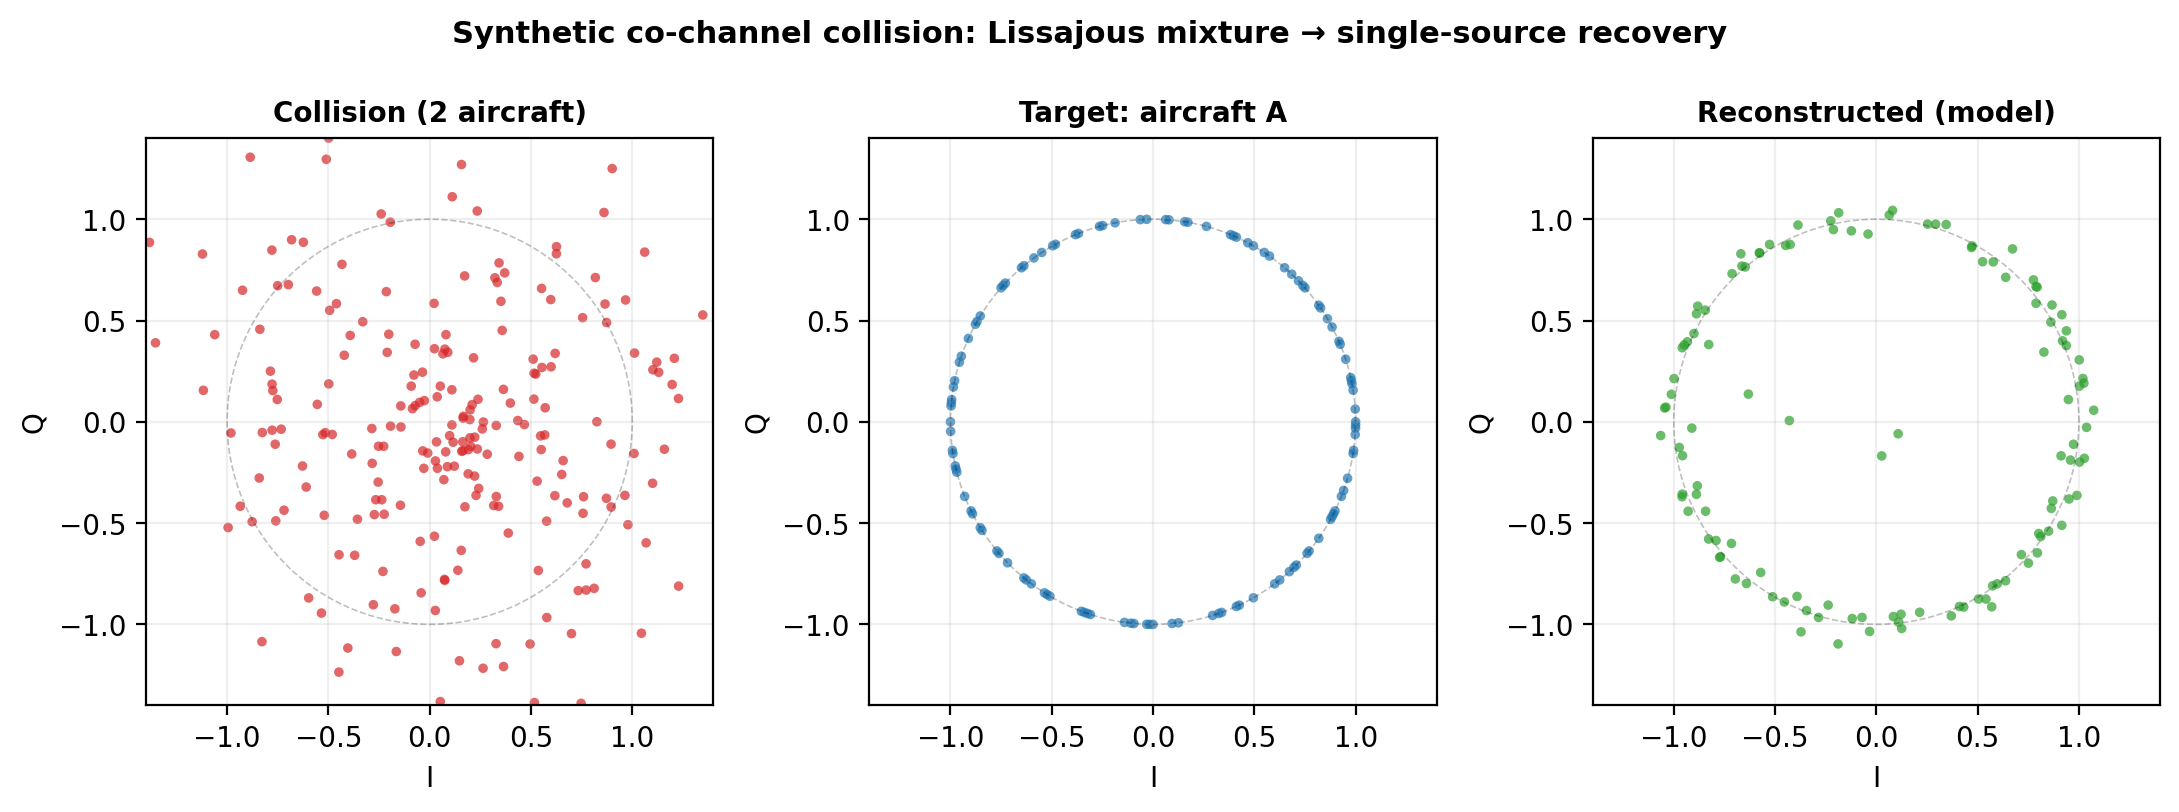
\includegraphics[width=\linewidth]{figures/fig_collision.png}
  \caption{Synthetic collision scenario: Lissajous mixture of two aircraft (left),
  clean target aircraft~A (centre), and model reconstruction (right). Generated
  with \texttt{checkpoints/best.pt} (synthetic pre-training).}
  \label{fig:collision}
\end{figure}

\subsection{Supervised Fine-Tuning (v1) --- Partial Real-World Success}

On \texttt{adsb\_capture.bin} (480~MB, 240M samples, in-distribution
benchmark):

\begin{table}[htbp]
  \centering
  \caption{v1 evaluation on in-distribution capture.}
  \label{tab:v1-results}
  \begin{tabular}{@{}lcccc@{}}
    \toprule
    Condition & Noise floor & Preamble cand. & Valid frames & Aircraft \\
    \midrule
    Raw & 0.110 & 25{,}371 & \textbf{1{,}589} & \textbf{31} \\
    Synthetic only (\texttt{best.pt}) & 0.507 & 3 & 0 & 0 \\
    Supervised v1 (\texttt{best\_supervised.pt}) & 0.069 & 16{,}097 &
    \textbf{116} & \textbf{17} \\
    \bottomrule
  \end{tabular}
\end{table}

v1 suppresses noise below the raw hardware floor (0.069 vs.\ 0.110) and
recovers 116 frames (7.3\% of raw)---establishing that domain-adapted
supervised training can produce downstream-decodable output, albeit with heavy
frame loss at full model strength.

\subsection{Training Iterations v2--v4 --- Validation Loss Anti-Correlates}

\begin{table}[htbp]
  \centering
  \caption{Checkpoint comparison on \texttt{adsb\_capture.bin} (full model,
  $\alpha=1$).}
  \label{tab:checkpoint-comparison}
  \begin{tabular}{@{}lcccc@{}}
    \toprule
    Checkpoint & Val loss & Collision aug & Frames & vs.\ raw \\
    \midrule
    v1 & 3.065 & none & \textbf{116} & 7.3\% \\
    v2 & 2.208 & 30\% clean interferer & \textbf{8} & 0.5\% \\
    v3 & improved & 10\% noisy interferer & 0 on OOD test$^*$ & --- \\
    v4 & 2.303 & 0\% & \textbf{83} & 5.2\% \\
    \bottomrule
  \end{tabular}
  \vspace{0.5em}
  \raggedright\small $^*$v3 evaluated on \texttt{test\_capture\_36db.bin};
  in-distribution benchmark on \texttt{adsb\_capture.bin} was not completed
  before experimental closure.
\end{table}

v2's lower loss accompanied \textbf{catastrophic decode regression} (8 vs.\ 116
frames). Root cause: the model learned to suppress clean structured patterns
from collision augmentation, then applied that behaviour to the primary
aircraft at inference. v4's denoising-only retrain further reduced loss but
still regressed versus v1.

\subsection{Out-of-Distribution Failure}

A 120~MB capture (\texttt{test\_capture\_36db.bin}, 30~s, 1090~MHz centre,
36~dB gain) with \textbf{314 raw CRC-valid frames} was held out as an OOD test:

\begin{table}[htbp]
  \centering
  \caption{OOD evaluation on \texttt{test\_capture\_36db.bin} ($\alpha=1$).}
  \label{tab:ood}
  \begin{tabular}{@{}lll@{}}
    \toprule
    Model & Valid frames & Notes \\
    \midrule
    Raw input & \textbf{314} & Strong baseline \\
    v1 & 0 & Works on \texttt{adsb\_capture.bin}, fails here \\
    v2 & 0 & Over-suppression \\
    v3 & 0 & Corrected augmentation insufficient \\
    v4 ($\alpha=1$) & 1 & Marginal; not meaningful \\
    \bottomrule
  \end{tabular}
\end{table}

Model outputs retain hundreds of preamble candidates but fail CRC---producing
plausible but subtly corrupted waveforms, not white noise.

\subsection{Pipeline Validation --- Infrastructure Is Not the Bottleneck}

\begin{table}[htbp]
  \centering
  \caption{Pipeline validation on \texttt{test\_capture\_36db.bin}.}
  \label{tab:pipeline-validation}
  \begin{tabular}{@{}lcc@{}}
    \toprule
    Condition & Valid frames & Aircraft \\
    \midrule
    Raw & \textbf{314} & 9 \\
    \texttt{--identity} (OLA/DC/RMS, no model) & \textbf{314} & 9 \\
    v1 model & 0 & 0 \\
    \bottomrule
  \end{tabular}
\end{table}

Overlap-add synthesis, global DC warmup, windowing, and RMS normalisation
preserve all decodable frames. Zero-frame failures are attributable to
\textbf{learned model weights}. A DC warmup fix was applied; on this capture DC
bias was ${\sim}0.1\%$ of full scale and did not change frame counts.

\subsection{Blend Diagnostic --- Deployable Partial Success}
\label{sec:blend}

Because full-strength model output over-suppresses real ADS-B structure, I
evaluated a post-hoc mix:
\begin{equation}
  \mathrm{out} = \alpha \cdot \mathrm{model} + (1 - \alpha) \cdot \mathrm{raw}.
  \label{eq:blend}
\end{equation}

Offline sweeps (\texttt{blend\_sweep.py}) and online streaming
(\texttt{live\_bridge.py --blend}) were cross-validated after fixing blend
buffer edge cases (Figures~\ref{fig:results-bars} and~\ref{fig:blend-sweep}).

\begin{figure}[htbp]
  \centering
  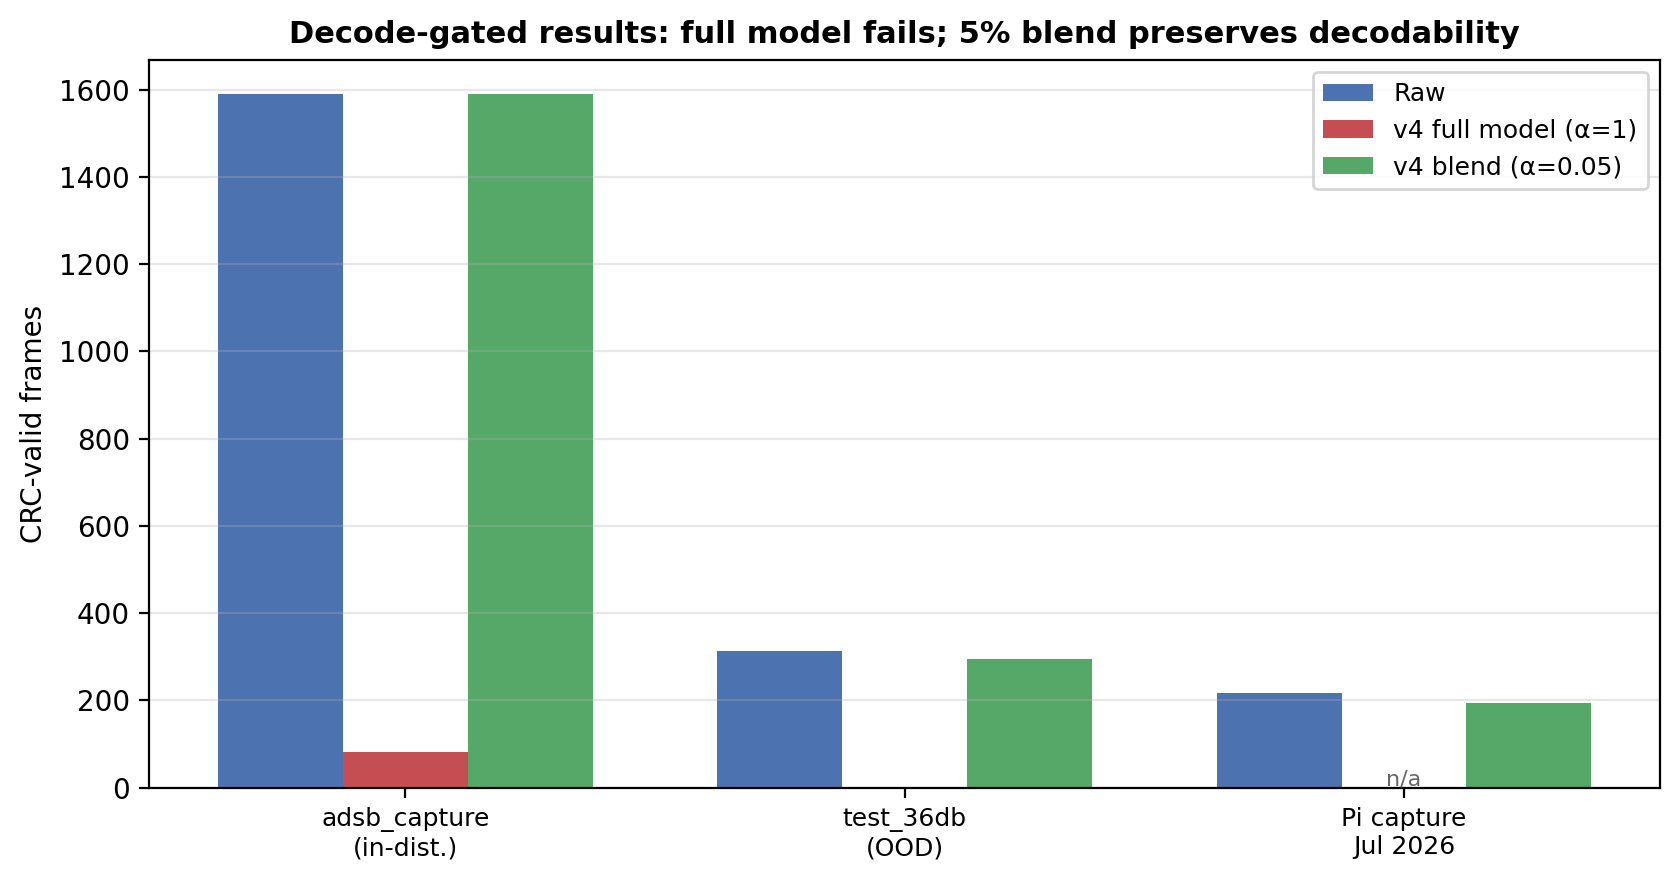
\includegraphics[width=0.88\linewidth]{figures/fig_results_bars.png}
  \caption{Decode-gated frame counts across three captures: raw input, v4 at
  full strength ($\alpha=1$), and v4 with 5\% model blend ($\alpha=0.05$).}
  \label{fig:results-bars}
\end{figure}

\begin{figure}[htbp]
  \centering
  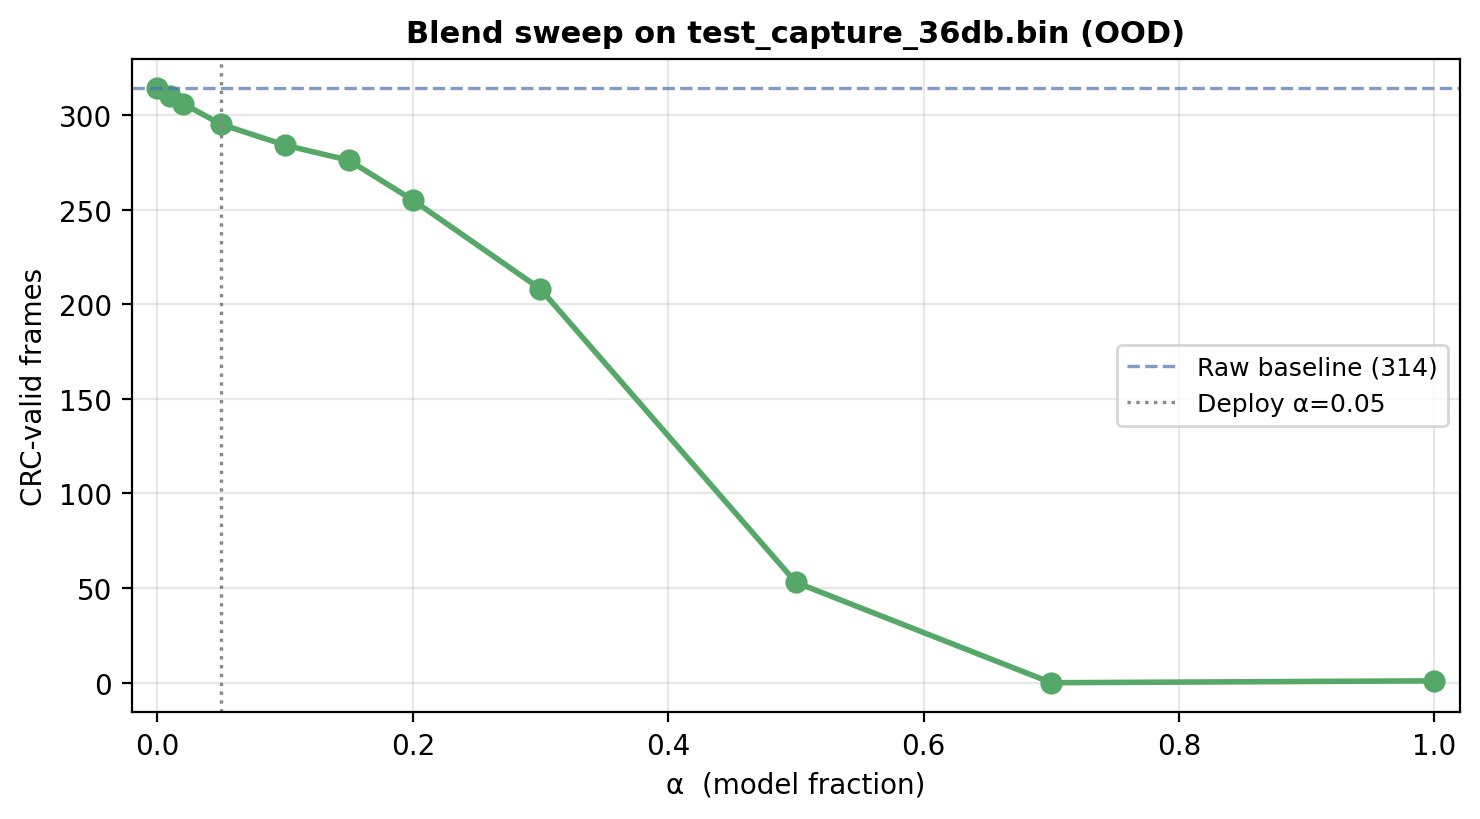
\includegraphics[width=0.82\linewidth]{figures/fig_blend_sweep.png}
  \caption{Blend sweep on \texttt{test\_capture\_36db.bin}: frame recovery falls
  sharply above $\alpha \approx 0.2$; $\alpha=0.05$ preserves 295/314 frames
  (93.9\%).}
  \label{fig:blend-sweep}
\end{figure}

\begin{table*}[htbp]
  \centering
  \caption{Master results table (decode-gated metric). Bold rows indicate
  deployable blend configuration.}
  \label{tab:master-results}
  \small
  \begin{tabular}{@{}llcccc@{}}
    \toprule
    Condition & Capture & Raw frames & Processed frames & Recovery \\
    \midrule
    Synthetic only & \texttt{adsb\_capture.bin} & 1{,}589 & 0 & 0\% \\
    v1 ($\alpha=1$) & \texttt{adsb\_capture.bin} & 1{,}589 & 116 & 7.3\% \\
    v2 ($\alpha=1$) & \texttt{adsb\_capture.bin} & 1{,}589 & 8 & 0.5\% \\
    v4 ($\alpha=1$) & \texttt{adsb\_capture.bin} & 1{,}589 & 83 & 5.2\% \\
    \textbf{v4 blend $\alpha=0.05$} & \texttt{adsb\_capture.bin} & 1{,}589 &
    \textbf{1{,}589} & \textbf{100\%} \\
    v1--v4 ($\alpha=1$) & \texttt{test\_capture\_36db.bin} & 314 & 0--1 &
    ${\sim}0\%$ \\
    \textbf{v4 blend $\alpha=0.05$} & \texttt{test\_capture\_36db.bin} & 314 &
    \textbf{295} & \textbf{93.9\%} \\
    \textbf{v4 blend $\alpha=0.05$} & \texttt{capture\_36db\_20260707} (Pi) &
    217 & \textbf{194} & \textbf{89.4\%} \\
    \bottomrule
  \end{tabular}
\end{table*}

The fresh Pi capture (\texttt{capture\_36db\_20260707\_145107.bin},
\texttt{rpi\_west}, 36~dB gain, 30~s) confirms blend behaviour on newly
collected data: 194/217 frames (11 aircraft in both raw and blended streams).

At $\alpha=0.05$, the model contributes 5\% of the output while raw preserves
95\%---sufficient to retain PPM structure for CRC validation. This is the
\textbf{only deployable configuration} identified in this study. It does not
demonstrate denoising benefit over raw; it demonstrates that the learned
representation is \textbf{directionally non-destructive} at low mixture weight.

%=============================================================================
\section{Discussion}
\label{sec:discussion}
%=============================================================================

\subsection{Structural Constraints}
\label{sec:constraints}

Three constraints block standalone full-strength deployment:

\textbf{No true clean RF reference.} Supervised targets are re-synthesised
ideal frames from decoded bits, not antenna-ground-truth waveforms. Multipath,
pulse shaping, and phase trajectory differences between target and reality
create a persistent train/serve gap.

\textbf{No real collision ground truth.} CRC-passing collisions are virtually
absent in labelled data. BSS capability depends on synthetic pre-training and
on-the-fly augmentation---neither captures independent noise, multipath, and
oscillator statistics of two real simultaneous transmitters.

\textbf{Training objective $\neq$ decoder metric.} IQ/magnitude/phase
reconstruction loss does not enforce PPM bit-edge fidelity required for CRC.
v2 proved this explicitly: best-ever val loss, worst decode regression. Lower
inferred noise floor does not imply better frame recovery.

\subsection{Two Distinct Failure Modes}

\begin{table}[htbp]
  \centering
  \caption{Failure mode taxonomy.}
  \label{tab:failure-modes}
  \begin{tabular}{@{}lll@{}}
    \toprule
    Problem & Symptom & Status \\
    \midrule
    A.\ Single-aircraft denoising & 0 frames OOD & Blocking \\
    B.\ BSS / collision separation & Cannot test on ordinary captures &
    Not reached \\
    \bottomrule
  \end{tabular}
\end{table}

\texttt{test\_capture\_36db.bin} contains 314 ordinary single-aircraft
decodes, not a controlled collision scenario. The immediate blocker is signal
destruction, not collision discrimination.

\subsection{Fixed IF and Domain Shift}

The deployed system tunes RTL-SDR to +250~kHz IF (1090250000~Hz). Encoder
filters learn matched responses for specific phasor rotation rates. Captures at
different centre frequencies (e.g., direct 1090~MHz) sit outside the learned
angular-velocity band. Combined with gain, site, and temperature variation,
supervised fine-tuning is \textbf{not universally transferable}.

\subsection{What Has Been Ruled Out}

\begin{table}[htbp]
  \centering
  \caption{Ruled-out failure hypotheses.}
  \label{tab:ruled-out}
  \begin{tabular}{@{}ll@{}}
    \toprule
    Hypothesis & Evidence \\
    \midrule
    OLA / windowing bug & \texttt{--identity}: 314/314 frames preserved \\
    DC removal as primary cause & DC $\approx 0.001$; fix unchanged count \\
    \texttt{uint8} conversion corruption & \texttt{--passthrough} and
    \texttt{--identity} both pass \\
    Model never works on real data & v1: 116 frames in-distribution \\
    \bottomrule
  \end{tabular}
\end{table}

\subsection{Implications for ML-for-RF Practice}

This project illustrates a common pitfall: optimising proxy reconstruction
metrics while the deployment metric is downstream task success. Validation loss
improved across v2 and v4 while decode performance regressed or stagnated. For
sub-microsecond pulse systems, \textbf{decode-gated checkpoint selection}
should be treated as a first-class training requirement, not a post-hoc
evaluation step.

%=============================================================================
\section{Deployment}
%=============================================================================

\subsection{Recommended Configuration}

Use checkpoint \texttt{checkpoints/best\_supervised\_v4.pt} with \textbf{5\%
model blend}:

\begin{lstlisting}[style=cli]
python live_bridge.py \
    --ckpt checkpoints/best_supervised_v4.pt \
    --blend 0.05 \
    --input data/captures/capture.bin \
    --output artifacts/clean_blend005.bin

python compare_decodings.py \
    data/captures/capture.bin artifacts/clean_blend005.bin
\end{lstlisting}

For live streaming to \texttt{dump1090}:

\begin{lstlisting}[style=cli]
rtl_sdr -f 1090000000 -s 2000000 -g 36 - \
  | python live_bridge.py --ckpt checkpoints/best_supervised_v4.pt --blend 0.05 \
  | dump1090 --ifile /dev/stdin --raw
\end{lstlisting}

\textbf{Expectation management:} At $\alpha=0.05$, output $\approx$ raw. The
model runs on the full stream but contributes minimally. Do not expect improved
frame counts over raw; expect \textbf{preserved} frame counts.

\subsection{Artifacts}

\begin{table}[htbp]
  \centering
  \caption{Deployment artifacts.}
  \label{tab:artifacts}
  \begin{tabular}{@{}ll@{}}
    \toprule
    Artifact & Description \\
    \midrule
    \texttt{checkpoints/best\_supervised\_v4.pt} & Recommended checkpoint \\
    \texttt{deploy\_adsb\_capture\_blend.bin} & In-distribution benchmark \\
    \texttt{deploy\_test\_capture\_blend005.bin} & OOD benchmark \\
    \texttt{blend\_sweep.py} & Offline $\alpha$ sweep utility \\
    \texttt{compare\_decodings.py} & CRC frame count evaluation \\
    \bottomrule
  \end{tabular}
\end{table}

%=============================================================================
\section{Conclusion}
%=============================================================================

I set out to build a phase-aware IQ autoencoder for ADS-B denoising and
co-channel blind source separation, operating within legacy decoder
constraints. The project succeeded in demonstrating IQ-phase BSS in synthetic
simulation; building a scalable real-world labelling and training pipeline over
406~GB of field captures; achieving partial downstream success at full model
strength on an in-distribution capture (116 frames, noise floor suppression
below raw); validating infrastructure correctness via identity-mode pipeline
testing; and finding a deployable conservative configuration (5\% model blend)
preserving 89--100\% of raw decodability across three captures.

The project did not succeed in full-strength denoising that matches or exceeds
raw decode rates; OOD generalisation to arbitrary gain, frequency, and site
conditions; real-world collision resolution; or aligning training loss with
decode success.

\textbf{Experimental phase is closed.} Further progress requires decoder-aware
loss functions, decode-gated checkpoint selection, target blending during
training (not just inference), and ultimately real collision captures with
ground truth---not additional epochs of IQ MSE against re-synthesised targets.

%=============================================================================
\section{Future Work}
%=============================================================================

\begin{enumerate}[leftmargin=*]
  \item \textbf{Decode-gated training} --- select checkpoints by CRC frame
        count on held-out captures, not val loss alone.
  \item \textbf{Target blending during training} --- optimise for the
        $\alpha=0.05$ deployment mixture directly.
  \item \textbf{Pulse-weighted loss} --- weight reconstruction at preamble and
        data pulse positions.
  \item \textbf{Capture metadata audit} --- stratify training by gain, site,
        and IF; quantify OOD boundaries.
  \item \textbf{Real collision data} --- dual-synchronised SDR capture or
        high-fidelity hardware-in-the-loop simulation matching RTL-SDR noise
        texture.
  \item \textbf{IF domain randomisation} --- train across centre-frequency
        offsets for hardware-agnostic deployment.
  \item \textbf{Edge optimisation} --- TorchScript, INT8 quantisation, reduced
        \texttt{base\_channels} for Pi real-time targets.
\end{enumerate}

%=============================================================================
\appendix
\section{Reproducibility}
%=============================================================================

\subsection{Evaluation Command}

\begin{lstlisting}[style=cli]
python compare_decodings.py RAW.bin PROCESSED.bin
\end{lstlisting}

Reports CRC-valid frame count, unique ICAO addresses, preamble candidates, and
estimated noise floor.

\subsection{Blend Sweep}

\begin{lstlisting}[style=cli]
python blend_sweep.py RAW.bin MODEL_OUTPUT.bin \
    --alphas 0,0.01,0.02,0.05,0.1,0.2,0.5,1.0
\end{lstlisting}

\subsection{Regenerate Paper Figures}

\begin{lstlisting}[style=cli]
cd docs && python generate_paper_figures.py
# or: cd docs && make figures
\end{lstlisting}

Outputs in \texttt{figures/}: pipeline, PPM grid, collision constellation,
results bar chart, and blend sweep plots.

\subsection{Key Source Files}

\begin{table}[htbp]
  \centering
  \caption{Repository file inventory.}
  \label{tab:files}
  \small
  \begin{tabular}{@{}ll@{}}
    \toprule
    File & Role \\
    \midrule
    \texttt{generator.py} & Synthetic frame and collision synthesis \\
    \texttt{model.py} & IQAutoencoder, PhaseAwareLoss \\
    \texttt{extract\_labels.py} & CRC-gated supervised pair extraction \\
    \texttt{supervised\_dataset.py} & Dataset + collision augmentation \\
    \texttt{train\_supervised.py} & Supervised fine-tuning \\
    \texttt{live\_bridge.py} & Streaming inference, blend, identity modes \\
    \texttt{compare\_decodings.py} & Downstream decode evaluation \\
    \texttt{blend\_sweep.py} & Offline $\alpha$ sweep \\
    \texttt{generate\_paper\_figures.py} & Publication figure generator \\
    \bottomrule
  \end{tabular}
\end{table}

\subsection{Capture Provenance}

\begin{table}[htbp]
  \centering
  \caption{Evaluation capture files.}
  \label{tab:captures}
  \begin{tabular}{@{}lll@{}}
    \toprule
    File & Duration & Notes \\
    \midrule
    \texttt{data/captures/adsb\_capture.bin} & 480~MB & In-distribution; 1{,}589 raw frames \\
    \texttt{data/captures/test\_capture\_36db.bin} & 120~MB, 30~s & OOD; 1090~MHz, 36~dB \\
    \texttt{data/captures/capture\_36db\_20260707\_145107.bin} & 30~s & Pi capture; 217 raw \\
    \bottomrule
  \end{tabular}
\end{table}

\subsection{Extended Implementation Notes}

Additional engineering detail---training commands, file inventory, collector
fixes, and milestone logs---is documented in
\texttt{WHITEPAPER\_BLUEPRINT.md} in the repository. That file is a
supplementary technical appendix; this report is self-contained for methods,
results, and conclusions.

%=============================================================================
\bibliographystyle{plainnat}
\bibliography{references}

\end{document}
